\documentclass[twocolumn]{article}
\usepackage{graphicx}
\begin{document}
\title{Practical Programming in C-language}
\author{Pelle Garbus, 20092716}
\date{\today}
\maketitle
\begin{abstract}
A) The built-in data types for numbers in C-language are discussed for a 16-bit system. B) The solution to exam problem 13 is seen in Figure \ref{fig-tan} that has been computed from the ordinary differential equation \ref{eq-ode}. The numerical solution matches the plot of the tangent function from the math.h library in the same range.
\end{abstract}



\section{Data types in C}
The website 'http://www.studytonight.com/c/ datatype-in-c.php' offers an excellent overview of the different data types. There are characters (is not considered to be a data representing a number, but the character itself is represented by a number), integer, float and void (the latter is an empty-type). The first three data types can be altered by so-called modifiers (signed/unsigned/short/long). For the float-type there are additional double and long double.

Seen below are tables of int (Table \ref{table-int}), float (Table \ref{table-float}) and char (Table \ref{table-char}) that include their modifiers. The numbers of bytes used (for a 16-bit system) is listed directly next to the variable type. Again note that char is not a type used for numbers, but included here for a complete picture of the amount of data used for the different types and their modifiers. All data have been copied from the above link.

\newpage
\begin{table}[h] \center 
\begin{tabular}{l|c}
Type, bytes				&	Range 							\\\hline
int, 2					&	-32,768 to 32767				\\
unsigned int, 2			&	0 to 65535						\\
short int, 1			&	-128 to 127						\\
long int, 4				&	-2,147,483,648 to 2,147,483,647	\\
unsigned long int, 4	&	0 to 4,294,967,295				
\end{tabular}
\caption{'int'-properties for a 16-bit computer.}
\label{table-int}
\end{table}

\begin{table}[h] \center
\begin{tabular}{l|c}
Type, bytes		&	Range 						\\\hline
Float, 4		&	3.4E-38 to 3.4E+38			\\
double, 8		&	1.7E-308 to 1.7E+308		\\
long double, 10	&	3.4E-4932 to 1.1E+4932
\end{tabular}
\caption{'float'-properties for a 16-bit computer.}
\label{table-float}
\end{table}

\begin{table}[h] \center
\begin{tabular}{l|c}
Type, bytes		&	Range 		\\\hline
char, 1			&	-128 to 127	\\
unsigned char, 1&	0 to 255	
\end{tabular}
\caption{'char'-properties for a 16-bit computer.}
\label{table-char}
\end{table}



\newpage
\section{Exam problem 13}
The solution has been found by following the GNU manual chapter 27 on ordinary differential equations. Given is the ordinary differential equation (ODE) of the tangent function
\begin{equation}
% \textrm{erf}(x) = \frac 2{\sqrt\pi} \int_0^x e^{-\tau^2}
y' = 1 + y(0)^2
\label{eq-ode}
\end{equation}
with the starting condition y(0) = 0. The implementation of the ODE is given in a helper function that specifies the next y-value for a current y-position. The GSL rutine gsl\_odeiv.h provides a system for which the user-defined differential equation, the jacobian (not used), the dimension (single dimensional) and additional parameters (none) are given as input. A driver is allocated that takes in the newly defined system, a step-algorithm (rk8pd choosen) a starting step size, absolute allowed error (and relative error). The differential equation can now be solved numerically by running the defined driver from a user-defined start and end values by a desired number of steps. The number of steps is not important since the step-algorithmn moves through the gradient space of the differential equation, and only continues if below a certain error level. Otherwise the internal step-size is reduced.


\section{Solution to Problem 13}

The tangens function has a asymtote for every x fulfilling $\frac{\pi}{2}$ - n$\pi$. As the tangens function is a periodic function, it is only necessary to consider the solution within two adjacent asymtotes, i.e. ]-$\frac{\pi}{2}$, $\frac{\pi}{2}$[. The solution to the exercise has only been carried out from [0,$\frac{\pi}{2}$[ due to symmetry arguments. Tangens is an odd function, i.e. f(-x) = -f(x), why the y values found in the positive range can directly be used in the range below x = 0 with a negative sign.

\begin{figure}[h]
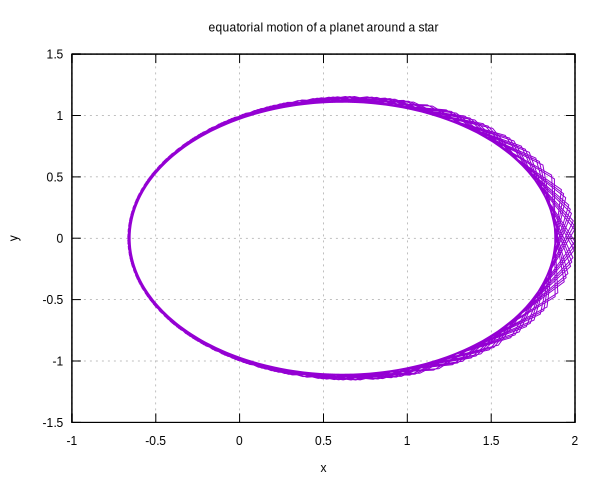
\includegraphics{plot.pdf}
\caption{The tangential function found by the differential equation \ref{eq-ode} and compared with the tangential function provided by the math.h library in the range [0,$\frac{\pi}{2}$[.}
\label{fig-tan}
\end{figure}

\end{document}